\subsection{Terrain Generator Architecture}
The architecture of our terrain generator is shown in Figure~\ref{fig:arch}. At the bottom sits the WebGL API, which is used to send shader programs to GPU. Three.js is built on WebGL API to hide details of shaders and provide a convenient way to manipulate the 3D scene. Then we developed several utility functions setup the scene and camera, as well as using the height map generated by above-mentioned algorithms to render terrains. We also develop extensions to three.js to produce richer effects. On top of them, we developed a simple API to be called from HTML page.
\begin{figure}
	\center
	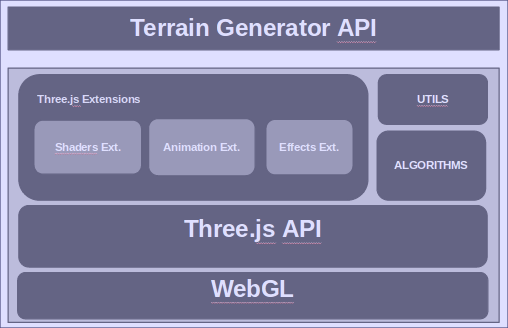
\includegraphics[scale=0.45]{images/arch.png}
	\caption{Architecture}
	\label{fig:arch}
\end{figure}
% subsection terrain generator architecture (end)
